

\begin{frame}{Introduction}
  \section{Introduction}
  \begin{columns}[T] 
    \begin{column}{0.5\textwidth}

      Here is some text 
      \begin{itemize}
        \item 
      \end{itemize}

    \end{column}
    \begin{column}{0.5\textwidth} 
      \begin{figure}
    \centering
    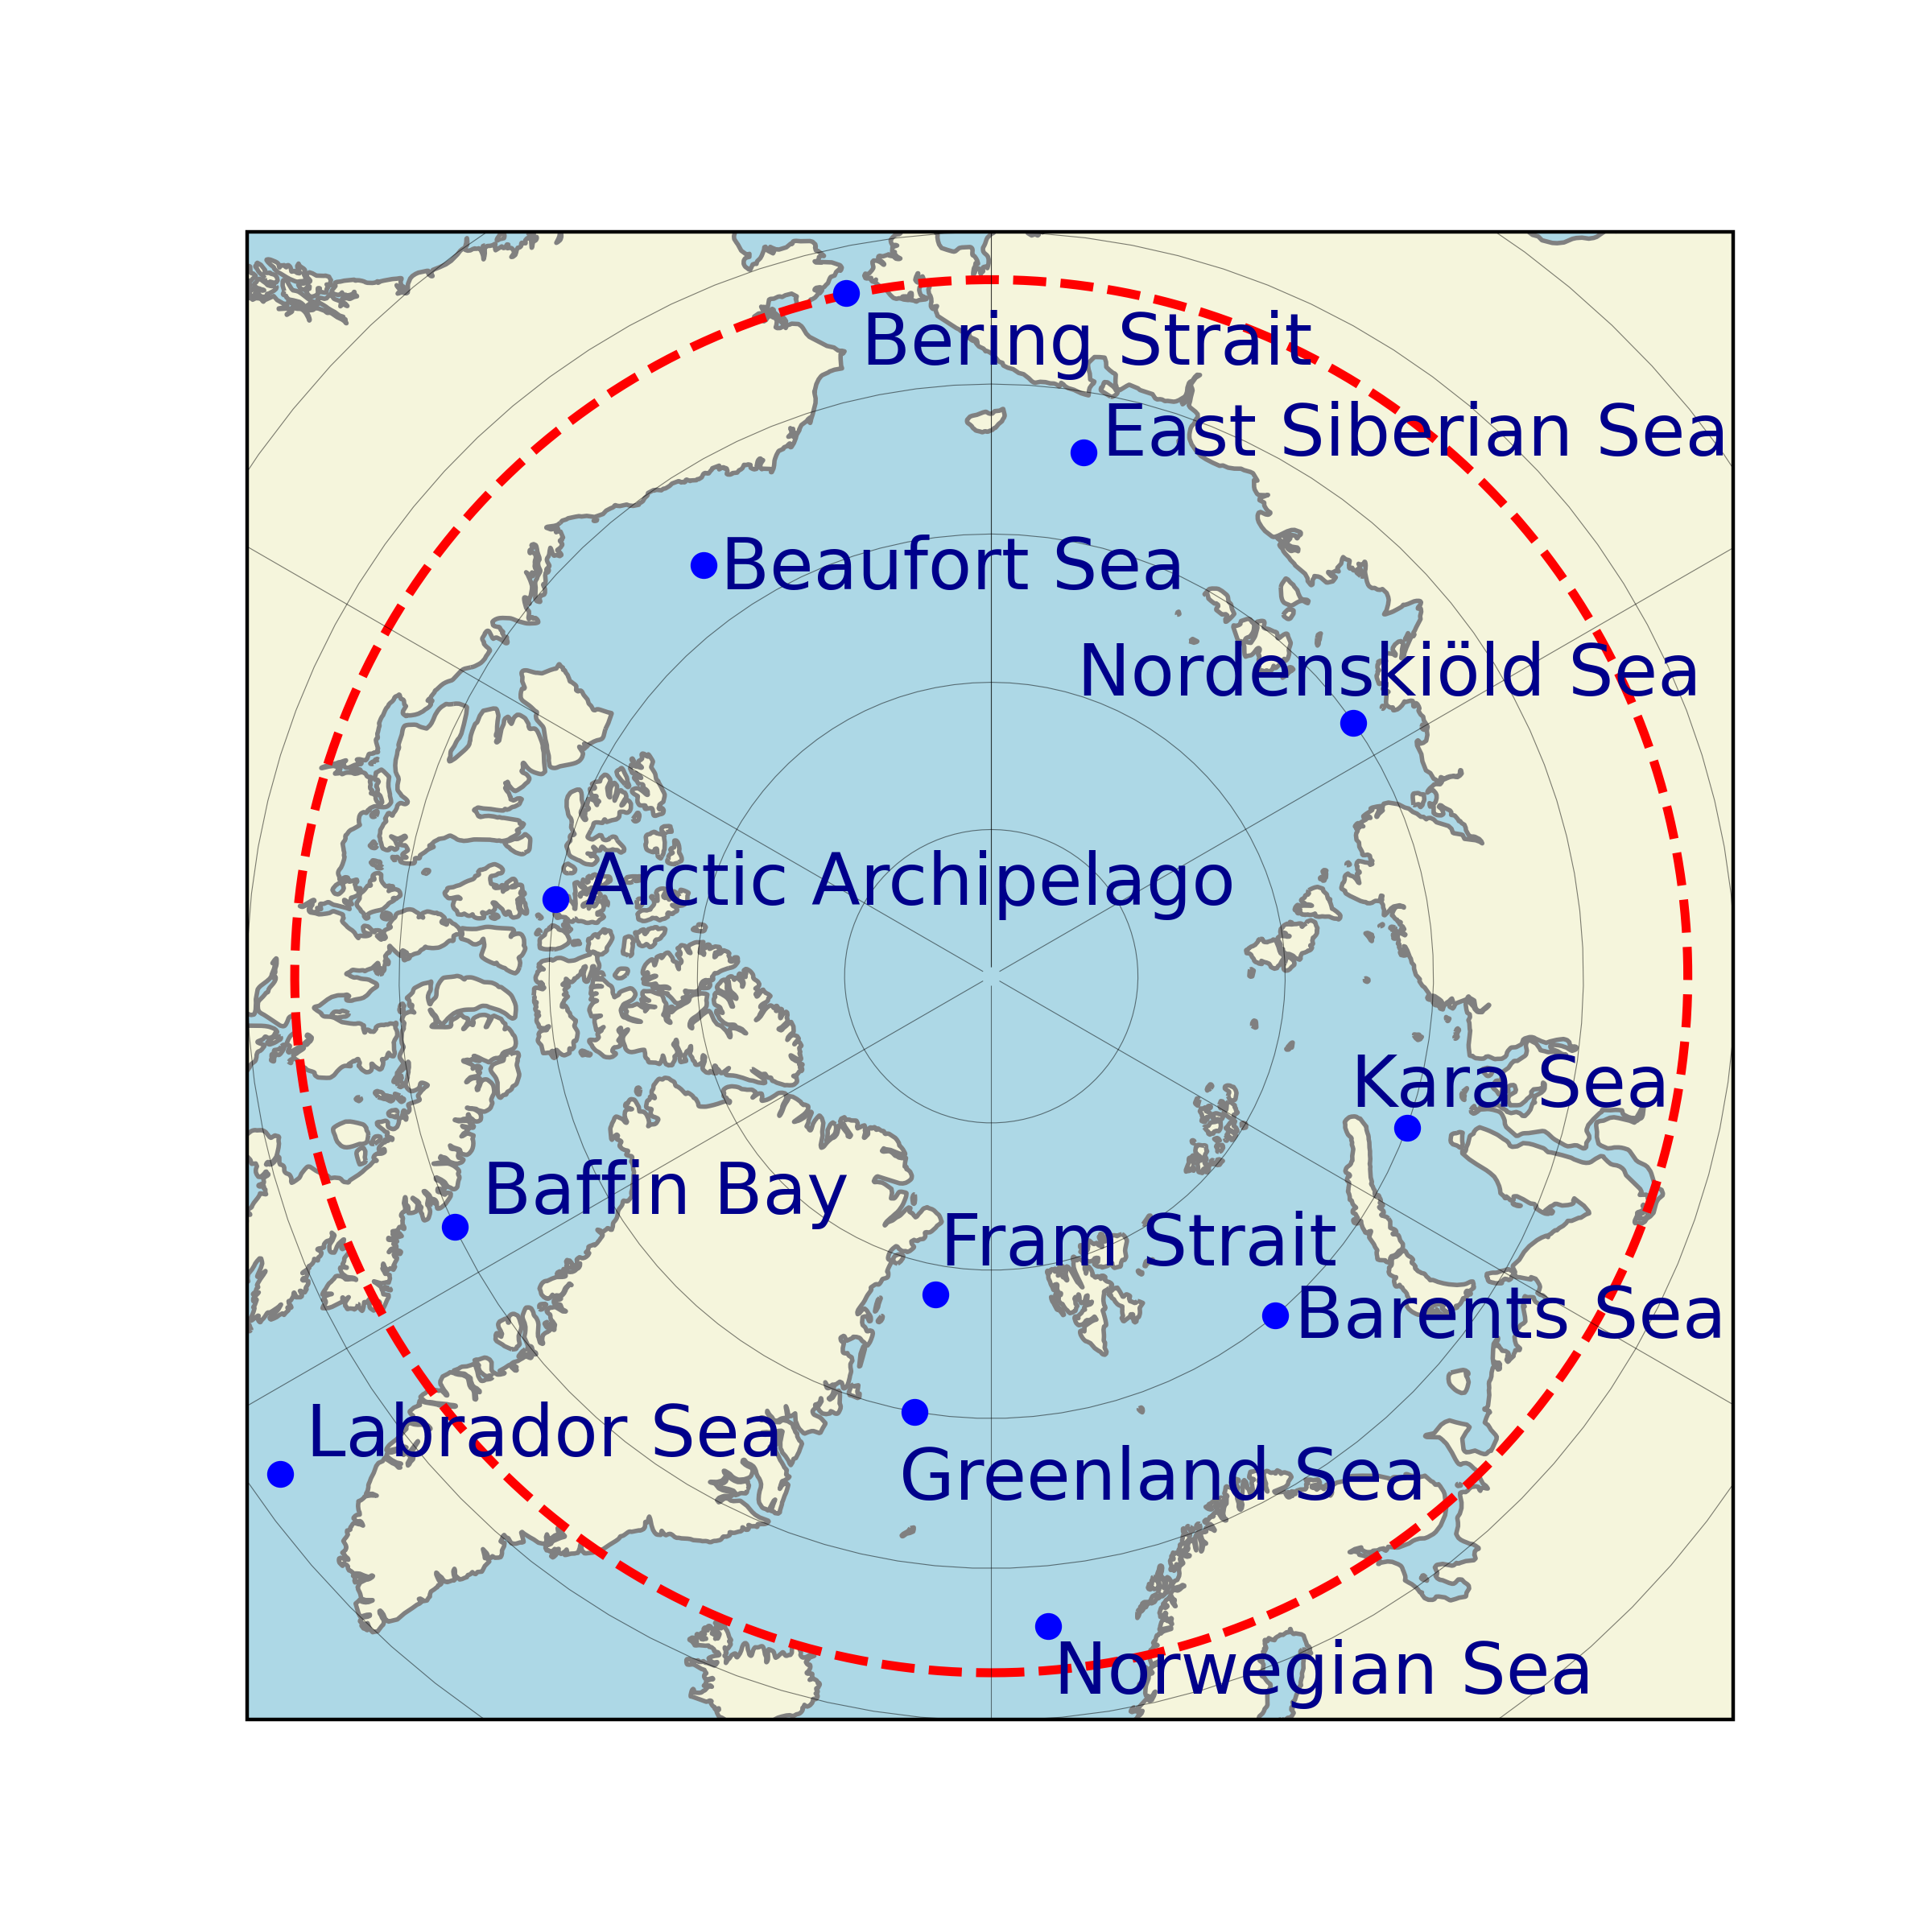
\includegraphics[width=\textwidth]{Figures/map.png}
    \caption{A map of the Arctic.}
  \end{figure}
    \end{column}
  \end{columns}
\end{frame}



\begin{frame}{Annual Means}
    \section{The regional climate}
    \begin{figure}
        \begin{subfigure}[b]{0.49\textwidth}
            \centering
            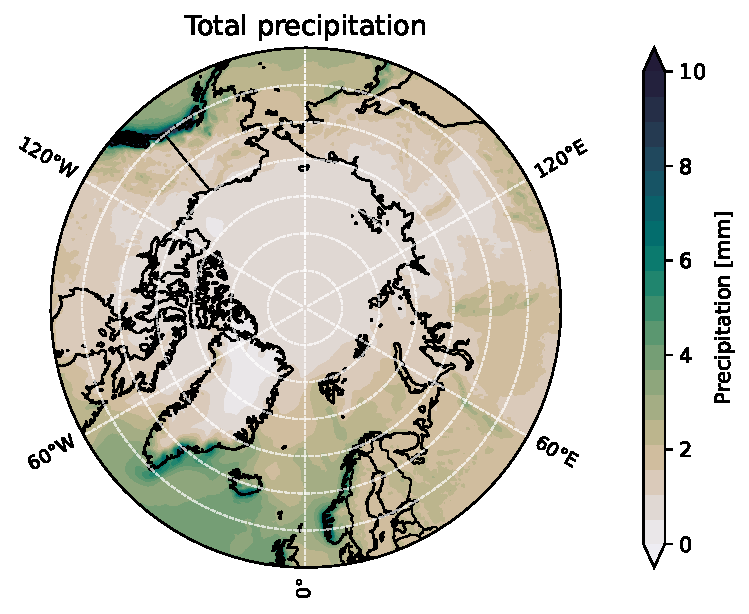
\includegraphics[height=0.4\textheight,keepaspectratio]{Figures/TotalPrecipitation_2012_2021_annual.pdf}
            \caption{Total Monthly Precipitation}
        \end{subfigure}
        \hfill
        \begin{subfigure}[b]{0.49\textwidth}
            \centering
            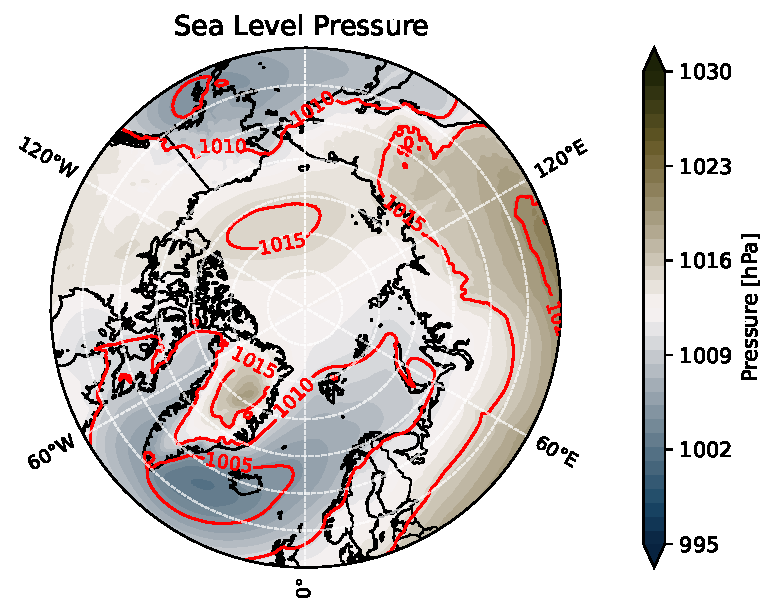
\includegraphics[height=0.4\textheight,keepaspectratio]{Figures/SeaLevelPressure_2012_2021_annual.pdf}
            \caption{Sea Level Pressure}
        \end{subfigure}
        \caption{Annual mean sea level pressure  and total monthly precipitation (2012--2021).}
    \end{figure}
\end{frame}

\begin{frame}{Monthly Means}
    \begin{figure}
        \begin{subfigure}[b]{0.49\textwidth}
            \centering
            
\includegraphics[height=0.4\textheight,keepaspectratio]{Figures/SeaLevelPressure_2012_2021_mean_DJF.pdf}
            \caption{Sea Level Pressure}
        \end{subfigure}
        \hfill
        \begin{subfigure}[b]{0.49\textwidth}
            \centering
            
\includegraphics[height=0.4\textheight,keepaspectratio]{Figures/SeaLevelPressure_2012_2021_mean_JJA.pdf}
            \caption{Sea Level Pressure}
        \end{subfigure}
        \caption{Monthly mean sea level pressure  (2012--2021).}
    \end{figure}
\end{frame}

\begin{frame}{Winter conditions}
    \begin{figure}
        \begin{subfigure}[b]{0.49\textwidth}
            \centering
            
\includegraphics[height=0.4\textheight,keepaspectratio]{Figures/Temperature_2012_2021_mean_DJF.pdf}
            \caption{Temperature}
        \end{subfigure}
        \hfill
        \begin{subfigure}[b]{0.49\textwidth}
            \centering
            
\includegraphics[height=0.4\textheight,keepaspectratio]{Figures/SeaIce_2012_2021_mean_DJF.pdf}
            \caption{Sea Ice}
        \end{subfigure}
    \end{figure}
\end{frame}

\begin{frame}{Spring conditions}
    \begin{figure}
        \begin{subfigure}[b]{0.49\textwidth}
            \centering
            
\includegraphics[height=0.4\textheight,keepaspectratio]{Figures/Temperature_2012_2021_mean_MAM.pdf}
            \caption{Temperature}
        \end{subfigure}
        \hfill
        \begin{subfigure}[b]{0.49\textwidth}
            \centering
            
\includegraphics[height=0.4\textheight,keepaspectratio]{Figures/SeaIce_2012_2021_mean_MAM.pdf}
            \caption{Sea Ice}
        \end{subfigure}
    \end{figure}
\end{frame}

\begin{frame}{Summer conditions}
    \begin{figure}
        \begin{subfigure}[b]{0.49\textwidth}
            \centering
            
\includegraphics[height=0.4\textheight,keepaspectratio]{Figures/Temperature_2012_2021_mean_JJA.pdf}
            \caption{Temperature}
        \end{subfigure}
        \hfill
        \begin{subfigure}[b]{0.49\textwidth}
            \centering
            
\includegraphics[height=0.4\textheight,keepaspectratio]{Figures/SeaIce_2012_2021_mean_JJA.pdf}
            \caption{Sea Ice}
        \end{subfigure}
    \end{figure}
\end{frame}

\begin{frame}{Autumn conditions}
    \begin{figure}
        \begin{subfigure}[b]{0.49\textwidth}
            \centering
            
\includegraphics[height=0.4\textheight,keepaspectratio]{Figures/Temperature_2012_2021_mean_SON.pdf}
            \caption{Temperature}
        \end{subfigure}
        \hfill
        \begin{subfigure}[b]{0.49\textwidth}
            \centering
            
\includegraphics[height=0.4\textheight,keepaspectratio]{Figures/SeaIce_2012_2021_mean_SON.pdf}
            \caption{Sea Ice}
        \end{subfigure}
    \end{figure}
\end{frame}

\begin{frame}{The Atmosphere}
  \section{The general circulation}
  
\end{frame}


\begin{frame}{The Ocean}
  \begin{columns}[T] 
    \begin{column}{0.6\textwidth} left
      Here is some text about the ocean:
      \begin{itemize}
        \item The ocean covers more than 70\% of the Earth's surface.
        \item It plays a crucial role in regulating the climate.
        \item The ocean is home to a vast array of marine life.
      \end{itemize}
    \end{column}
    \begin{column}{0.4\textwidth} 
      \begin{figure}
        \centering
        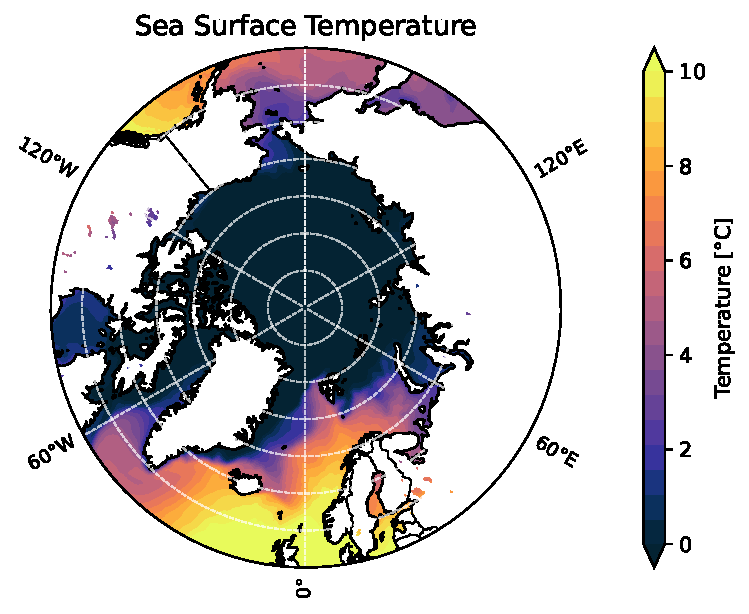
\includegraphics[width=\textwidth]{Figures/SeaSurfaceTemperature_2012_2021_annual.pdf}
        \caption{Sea Surface Temperature (2012--2021)}
      \end{figure}
    \end{column}
  \end{columns}
\end{frame}




\begin{frame}{Climate Change}
    \section{Climate Change}
  Your content here \citep{serreze2014}
\end{frame}


\begin{frame}{Societal activities}
    \section{Societal activities}
  Your content here \citep{serreze2014}
\end{frame}